%\documentclass{slides}
\documentclass{beamer}
\usepackage[utf8]{inputenc}
%\usepackage{portland}
\usepackage{graphicx}
%\usepackage{pdflscape}

%========Hierboven niets veranderen!========%

\usepackage[export]{adjustbox}% for the second solution
\usepackage{amsmath}
\usepackage{amsfonts}
\usepackage{amssymb}
\usepackage{mathtools}
\usepackage{scalerel}
\usepackage[normalem]{ulem}
\usepackage{wisjab}

\setlength\fboxsep{4mm}
\setlength\fboxrule{0.8mm}

\definecolor{mygreen}{rgb}{0, 0.5, 0}
\def\gemph#1{{\color{mygreen}#1}}
\def\ck{\cellcolor{green!05}}

\def\lbt{\small QC$^2$ meeting 29-04-2024} %Titel die linksboven verschijnt
\parindent=0pt
%\makesavenoteenv{tabular}
\renewcommand{\thefootnote}{\arabic{footnote}}

\DeclareMathOperator{\tr}{tr}
\DeclareMathOperator{\sgn}{sgn}
\DeclareMathOperator{\poly}{poly}
\DeclareMathOperator{\polylog}{polylog}
\DeclareMathOperator{\Rea}{Re}
\DeclareMathOperator{\Ima}{Im}
\renewcommand{\Re}{\Rea}
\renewcommand{\Im}{\Ima}

\def\vc#1{\boldsymbol{\mathsf{#1}}}
\def\mt#1{\kern0.025em\mathsf{#1}\kern0.025em}
\def\mtg#1{\kern0.6pt\slantbox[-0.25]{$#1$}\kern-0.6pt}

\def\1{\mathds1}
\def\d{\mathsf d}
\def\e{\mathsf e}
\def\i{\mathsf i}
\def\lambdai{{\lambda_{\sf i}}}
\def\lambdaf{{\lambda_{\sf f}}}

\def\A{\mt A}
\def\H{\mt H}
\def\HCD{\mt H_{\sf CD}}
\def\U{\mt U}

\def\+{\kern0.0833em}
\def\:{\kern-0.07em}
\def\>{\kern0.08em}
\def\<{\kern-0.08em}

\renewcommand{\thefootnote}{\arabic{footnote}}

\newenvironment{dia}[2]
{
	\begin{frame}
	\vspace{1mm}
	{\small #1}
	\hfill
    {\small\bf\textcolor{blue}{#2}}
	\vspace{3mm}
	\hrule
	\bigskip
}
{
	\vfill
	\end{frame}
}

\frenchspacing

\begin{document}

\setlength{\abovedisplayskip}{3mm}
\setlength{\belowdisplayskip}{3mm}
\setlength{\abovedisplayshortskip}{3mm}
\setlength{\belowdisplayshortskip}{3mm}

\begin{dia}{\lbt}{}
\vspace*{0.5cm}
\begin{center}
\begin{large}
QC$^2$ meeting 29-04-2024 \\[1.25cm]
\end{large}
\begin{LARGE}
\textcolor{mygreen}{Gate-based counterdiabatic driving with complexity guarantees} \\[1.25cm]
\end{LARGE}
Dyon van Vreumingen
\end{center}
\end{dia}

\begin{dia}{\lbt}{Contents}
$ $\\
\begin{itemize}
    \setlength{\itemsep}{3mm}
    \item Adiabatic state preparation (ASP) and counterdiabatic driving (CD) \pause
    \item Hardness of CD and need for fair comparison with ASP \pause
    \item Gate-based CD algorithm and complexity bounds \pause
    \item Conclusion and outlook
\end{itemize}
\vspace{2.4cm}
\end{dia}

\begin{dia}{\lbt}{}
\vspace{2.5cm}
\begin{center}
\begin{LARGE}
\textcolor{mygreen}{Adiabatic state preparation and counterdiabatic driving}
\end{LARGE}
\end{center}
\vspace*{1.5cm}
\end{dia}

\begin{dia}{\lbt}{Adiabatic state preparation}
Given: \pause
\begin{itemize}
    \item family of continuously parametrised hamiltonians $\H(\lambda)$ \pause
    \item system prepared in eigenstate $\ket{n(\lambdai)}$ of $\H(\lambdai)$ for some $\lambdai$ \pause
\end{itemize}
$ $\\[-2mm]
Objective: find corresponding eigenstate (ground state) of $\H(\lambdaf)$ for some $\lambdaf$ \pause \\[4mm]
Example: $\H(\lambda) = \mt h + \lambda \mt V$, $\lambdai = 0$, $\lambdaf = 1$ \pause \\[4mm]
\gemph{Adiabatic theorem}: \pause
\begin{itemize}
    \item slowly (and continuously) vary $\lambda$ with time, such that $\lambda(t=0) = \lambdai$ and $\lambda(t=T) = \lambdaf$ \pause
    \item time-evolved state w.r.t. time-dependent hamiltonian $\H(\lambda(t))$ approximates $\ket{n(\lambdaf)}$
\end{itemize}
\vspace{-1cm}
\end{dia}

\begin{dia}{\lbt}{Adiabatic state preparation}
$ $ \\[7mm]
\begin{center}
    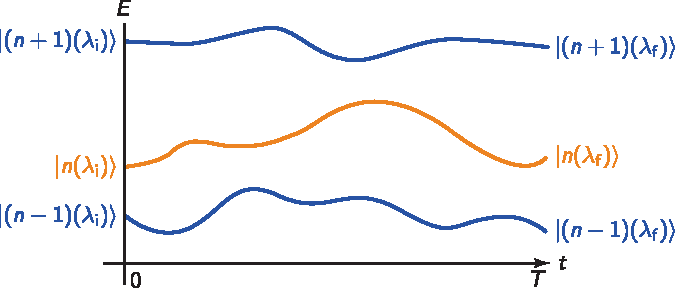
\includegraphics[width=\textwidth]{fig/adiabatisch_a.pdf}
\end{center}
\vspace{-1cm}
\end{dia}

\begin{dia}{\lbt}{Adiabatic state preparation}
$ $ \\[7mm]
\begin{center}
    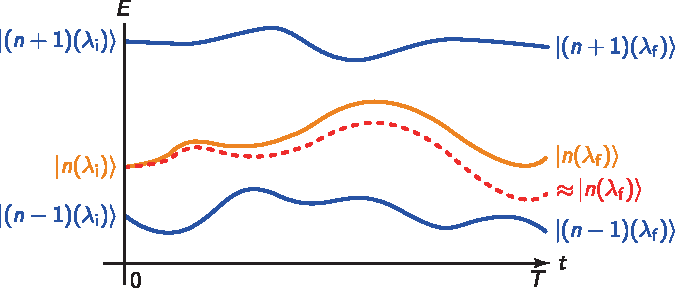
\includegraphics[width=\textwidth]{fig/adiabatisch_b.pdf}
\end{center}
\vspace{-1cm}
\end{dia}

\begin{dia}{\lbt}{Adiabatic state preparation}
$ $ \\[7mm]
\begin{center}
    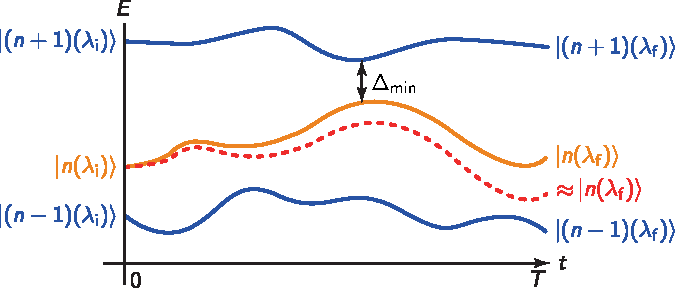
\includegraphics[width=\textwidth]{fig/adiabatisch_c.pdf}
\end{center}
\vspace{-1cm}
\end{dia}

\begin{dia}{\lbt}{Counterdiabatic driving}
Infidelity caused by \gemph{nonadiabatic transitions} into other eigenstates \pause \\[4mm]
Idea: time-evolve with $\HCD(t) = \H(t) + \text{something}(t)$ such that transitions are suppressed and we can evolve faster \pause \\[6mm]
\begin{center}
    \begin{tabular}{ccc}
        adiabatic & non-adiabatic & counter-diabatic \\[2mm]
        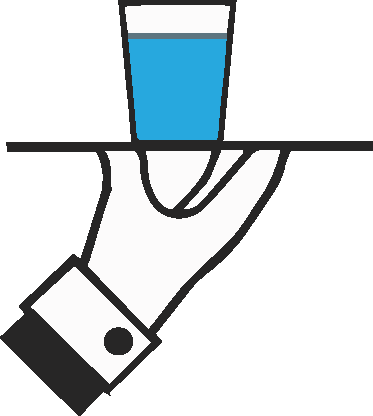
\includegraphics[scale=0.4]{fig/ober_a.pdf} &
        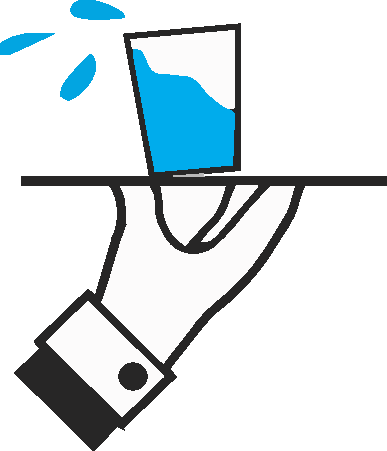
\includegraphics[scale=0.4]{fig/ober_b.pdf} &
        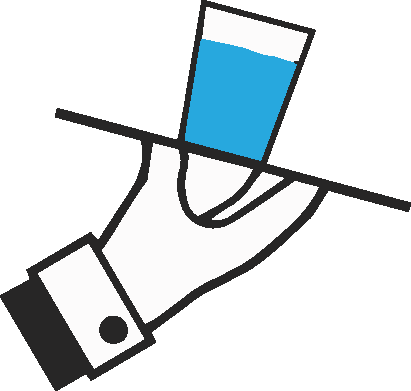
\includegraphics[scale=0.4]{fig/ober_c.pdf}
    \end{tabular}
\end{center}
\vspace{-1cm}
\end{dia}

\begin{dia}{\lbt}{Counterdiabatic driving}
Time-dependent Schr\"odinger equation:
\begin{align*}
    \i \+ \d_t \ket{n(\lambda(t))} = \H(\lambda(t)) \ket{n(\lambda(t))}
\end{align*} \pause
Define $\U(\lambda)$ such that $\U(\lambda) \ket{n(\lambdai)} = \ket{n(\lambda)}$ \pause \\[4mm]
Change to rotating frame that moves with eigenstates:
\begin{align*}
    \i \+ \d_t \ket{n} = [\mt U\t \mt H \mt U {\color{red} {} - \i \+ \dot\lambda \+ \mt U\t \partial_\lambda \mt U}] \ket{n}
\end{align*}
$ $ \pause \\[-2mm]
If we instead evolve with $\U\t\HCD\U := \U\t\H\U {\color{red} {} + \i \+ \dot\lambda \+ \mt U\t \partial_\lambda \mt U}$, then $\ket n$ remains \gemph{stationary} in rotating frame \pause \\[4mm]
In lab frame, $\HCD := \H + \i \+ \dot\lambda \+ \partial_\lambda \mt U \mt U\t$ suppresses all transitions
\vspace{-1cm}
\end{dia}

\begin{dia}{\lbt}{Counterdiabatic driving}
Operator $\A := \i \+ \partial_\lambda \mt U \mt U\t$ is known as \gemph{adiabatic gauge potential} \pause \\[4mm]
It is simply the derivative operator $\i \+ \partial_\lambda$:
\begin{align*}
    \bra{m(\lambda)} \mt A \ket{n(\lambda)} &= \i \+ \bra{m(\lambda)} \partial_\lambda \mt U \ket{n(\lambdai)} \\
    &= \i \+ \bra{m(\lambda)} \partial_\lambda \ket{n(\lambda)}
\end{align*} \pause
If we know $\A(\lambda)$, we can perform \gemph{transitionless} driving for \gemph{any driving time $T$} (i.e. also in limit $T\to0$)! \pause
\begin{align*}
    \sum_n \ket{n(\lambdaf)}\bra{n(\lambdai)} = \mathcal T\exp \bigg[ \!-\!\i \int_0^{{\color{mygreen}T}} \d t \, [\mt H(\lambda(t)) + \dot\lambda(t) \mt A(\lambda(t))] \bigg]
\end{align*}
\vspace{-1cm}
\end{dia}

\begin{dia}{\lbt}{Counterdiabatic driving}
Operator $\A := \i \+ \partial_\lambda \mt U \mt U\t$ is known as \gemph{adiabatic gauge potential} \\[4mm]
It is simply the derivative operator $\i \+ \partial_\lambda$:
\begin{align*}
    \bra{m(\lambda)} \mt A \ket{n(\lambda)} &= \i \+ \bra{m(\lambda)} \partial_\lambda \mt U \ket{n(\lambdai)} \\
    &= \i \+ \bra{m(\lambda)} \partial_\lambda \ket{n(\lambda)}
\end{align*}
If we know $\A(\lambda)$, we can perform \gemph{transitionless} driving for \gemph{any driving time $T$} (i.e. also in limit $T\to0$)!
\begin{align*}
    \sum_n \ket{n(\lambdaf)}\bra{n(\lambdai)} = \mathcal T\exp \bigg[ \!-\!\i \int_\lambdai^\lambdaf \d\lambda \, \mt A(\lambda) \bigg]
\end{align*}
\vspace{-1cm}
\end{dia}

\begin{dia}{\lbt}{Hardness of CD}
However, computing $\mt A$ is \gemph{hard}! \pause \\[2mm]
Methods to approximate AGP for imperfect but improved driving \pause
\begin{itemize}
    \item Variational methods:
    \begin{itemize}
        \item parametrised operator ansatz $\mt X(\vcg\alpha)$
        \item minimise action function $S(\mt X(\vcg\alpha))$
        %\item if $S(\mt X) = 0$, then $\mt X = \mt A$
        \item evaluating $S$ can take exponential time depending on ansatz
    \end{itemize} \pause
    \item Nested commutator / Krylov space methods: \vspace{-3mm}
    \begin{align*}
        \mt A^{(\ell)}_{\vcg\alpha} = \i \sum_{k=1}^{\ell} \alpha_k \underbrace{[\mt H, [\mt H, \ldots[\mt H}_{2k-1}, \partial_\lambda \mt H] \cdots ]]
    \end{align*}
    \vspace{-4mm}
    \begin{itemize}
        \item optimal $\alpha^*_k$ found through linear system of $\ell$ equations
        \item for chaotic (non-integrable) systems, $\ell \sim \mathrm{dim}(\mathcal H)^2$ required
    \end{itemize}
\end{itemize}
\vspace{-1cm}
\end{dia}

\begin{dia}{\lbt}{Hardness of CD}
This begs the question: \pause
\begin{center}
    \gemph{is counterdiabatic driving really worthwhile?} \pause
\end{center}
By this we mean:
\begin{itemize}
    \item does the computational complexity needed to boost fidelity through CD scale favourably... \pause
    \item ...as compared to simply increasing the evolution time in ASP?
\end{itemize} \pause
This question has so far been left unaddressed... \\[4mm] \pause
We should make a fair comparison between ASP and CD \\[4mm] \pause
We consider complexity in terms of quantum gates on fault-tolerant QC
\vspace{-1cm}
\end{dia}

\begin{dia}{\lbt}{Complexity of ASP}
%Denote $\|\mt O\|_{\infty, p} = \big( \int_\lambdai^\lambdaf \d\lambda \, \|\mt O(\lambda)\|^p \big)^{1 / p}$. Then f
For ASP, we know the the JRS bound
\begin{align*}
    T \geq O(\Delta^{-3} \epsilon^{-1} 
    %\|\partial_\lambda \mt H\|_{\infty, 2}^2
    ) \Rightarrow |\braket{n(\lambdaf)}{\psi(T)}|^2 \geq 1 - \epsilon^2
\end{align*}
where $\Delta$ is the minimum gap around $\ket{n(\lambda)}$ along the path \\[4mm] \pause
Combine this with state-of-the-art time-dependent Hamiltonian simulation techniques, to obtain that
\begin{align*}
    \tilde O(\Delta^{-3} \epsilon^{-1}
    %\|\mt H\|_{\infty, \infty} \|\partial_\lambda \mt H\|_{\infty, 2}^2
    )
\end{align*}
quantum gates are sufficient to obtain fidelity $\geq 1 - \epsilon^2$, where $\tilde O(f) = O(f \polylog(f))$
\vspace{-1cm}
\end{dia}

\begin{dia}{\lbt}{}
\vspace{2.5cm}
\begin{center}
\begin{LARGE}
\textcolor{mygreen}{Gate-based counterdiabatic driving}
\end{LARGE}
\end{center}
\vspace*{1.5cm}
\end{dia}

\begin{dia}{\lbt}{Gate-based CD}
Goal: to approximate the unitary
\begin{align*}
    \mt U(\lambdai, \lambdaf) = \sum_n \ket{n(\lambdaf)}\bra{n(\lambdai)} = \mathcal T \exp \bigg[ \! -\!\i \int_\lambdai^\lambdaf \d\lambda \, \mt A(\lambda)) \bigg]
\end{align*}
with some unitary $\tilde{\mt U}(\lambdai, \lambdaf)$ that can be implemented on a fault-tolerant QC \\[4mm] \pause
We will upper bound $\|(\mt U - \tilde{\mt U})\ket{n(\lambdai)}\|$, since
\begin{align*}
    \|(\mt U&(\lambdaf, \lambdai) - \tilde{\mt U}(\lambdaf, \lambdai))\ket{n(\lambdai)}\| \leq \epsilon \nonumber \\[2mm]
    &\Rightarrow |\bra{n(\lambdai)} \mt U\t(\lambdaf, \lambdai) \tilde{\mt U}(\lambdaf, \lambdai) \ket{n(\lambdai)}|^2 \geq 1 - \epsilon^2
\end{align*}
\vspace*{-1.4cm}
\end{dia}

\begin{dia}{\lbt}{Time-integral AGP}
By the Hellman-Feynman theorem,
\begin{align*}
    \bra m \A \ket n = -\i \bra m \partial_\lambda \ket n = \frac{\bra m \partial_\lambda\H \ket n}{\i \+ \omega_{mn}} \quad \quad \omega_{mn} = E_m - E_n
\end{align*} \pause
If we take
\begin{align*}
    \A = \frac12 \lim_{\eta\to0} \int_{-\infty}^\infty \d\tau \, \e^{-\eta|\tau|} \sgn(\tau) \, \e^{-\i\H\tau} \partial_\lambda \H \+ \e^{\i\H\tau} \\[-8mm]
\end{align*} \pause
then
\begin{align*}
    \bra m \A \ket n &= \frac12 \lim_{\eta\to0} \int_{-\infty}^\infty \d\tau \, \e^{-\eta|\tau|} \sgn(\tau) \, \e^{-\i(E_m - E_n)\tau} \bra m \partial_\lambda \H \ket n \\[2mm]
    &= \lim_{\eta\to0} \frac{\omega_{mn}}{\i(\omega_{mn}^2 + \eta^2)} \bra m \partial_\lambda \mt H \ket n
\end{align*}
%$\hat f(\omega) = \frac{\omega}{\i(\omega^2 + \eta^2)}$ has inverse FT $f(\tau) = \frac12 \e^{-\eta\tau} \sgn(\tau)$ \pause
\vspace{-1.4cm}
\end{dia}

\begin{dia}{\lbt}{Algorithm}
We construct a gate-based algorithm in three steps \pause
\begin{enumerate}
    \item Regularise and truncate integral expression:
    \begin{align*}
        \A \approx \A_{\eta, a} = \frac12 \int_{-a}^a \d\tau \, \e^{-\eta|\tau|} \sgn(\tau) \, \e^{-\i\H\tau} \partial_\lambda \H \+ \e^{\i\H\tau}
    \end{align*}
    for $\eta, a \geq 0$ \pause
    \item Approximate the time integral with a sum:
    \begin{align*}
        \A_{\eta, a}(\lambda) \approx \A_{\eta, a}^{M, q}(\lambda) = \sum_{\kappa = -M}^M \sum_{\alpha = 0}^q \mt C_{\kappa, \alpha}(\lambda)
    \end{align*}
\end{enumerate}
\vspace{0.65cm}
\end{dia}

\begin{dia}{\lbt}{Algorithm}
We construct a gate-based algorithm in three steps
\begin{enumerate}
    \setcounter{enumi}{2}
    \item Approximate time-ordered exponential
    \begin{align*}
        \mt U_{\eta, a}^{M, q}(\lambdaf, \lambdai) = \mathcal T \exp\big[ \!-\!\i \int_\lambdai^\lambdaf \d\lambda \, \A_{\eta, a}^{M, q}(\lambda) \big]
    \end{align*}
    with a Lie-Suzuki-Trotter (LST) formula
    \begin{align*}
        \mt U_{\eta, a}^{M, q}(\lambdaf, \lambdai) \approx \tilde{\mt U}(\lambdaf, \lambdai) = \prod_i \exp[-\i \> \mt C_{\kappa_i, \alpha_i}(\lambda_i) \> \delta\lambda_i]
    \end{align*}
\end{enumerate} \pause
By a triangle equality, the total error is then at most
\begin{align*}
    \|(\mt U - \tilde{\mt U})\ket{n(\lambdai)}\| &\leq \|(\mt U - \mt U_{\eta, a})\ket{n(\lambdai)}\| \\
    &+ \|(\mt U_{\eta, a} - \mt U_{\eta, a}^{M, q})\ket{n(\lambdai)}\| + \|(\mt U_{\eta, a}^{M, q} - \tilde{\mt U})\ket{n(\lambdai)}\|
\end{align*}
\vspace{-1cm}
\end{dia}

\begin{dia}{\lbt}{1. Regularisation and truncation}
Regularisation
\begin{align*}
    \bra m \A_{\eta, \infty} \ket n = \frac{\omega_{mn}}{\i (\omega_{mn}^2 + \eta^2)} \quad \quad \omega_{mn} = E_m - E_n
\end{align*}
has effect of suppressing only those transitions with $|\omega_{mn}| \gg \eta$ \\[4mm] \pause
But we need to suppress only the transitions from the $n$-th energy level! \\[4mm] \pause
Truncation introduces an additional error $\sim \e^{-\eta a}$; this leads to
\begin{align*}
    \eta &\leq O(\Delta^{3/2}\epsilon^{1/2}), \quad a \geq \tilde O(1 / \eta) \\[2mm]
    & \Rightarrow \|(\mt U - \mt U_{\eta, a})\ket{n(\lambdai)}\| \leq \epsilon
\end{align*}
\vspace{-1cm}
\end{dia}

\begin{dia}{\lbt}{2. Weighted sum approximation}
Riemann sum \pause
\begin{center}
    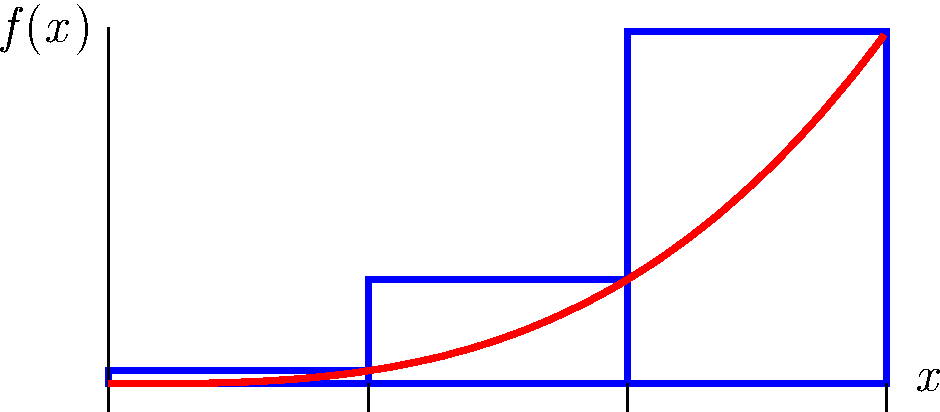
\includegraphics[width=0.7\textwidth]{fig/RightRiemann.pdf}
\end{center} \pause
\vspace{-2mm}
\begin{align*}
    \mt A_{\eta, a}^{M, 0} = \frac12 \sum_{\kappa = -M}^M \delta\tau_\kappa \> \e^{-\eta|\tau_\kappa|} \sgn\tau_\kappa \> \e^{-\i \mt H \tau_\kappa} \partial_\lambda \mt H \> \e^{\i \mt H \tau_\kappa}
\end{align*} \pause
\vspace{-2mm}
\begin{align*}
    M \geq O(\eta^{-2} \epsilon^{-1}) \Rightarrow \|(\mt U_{\eta, a} - \mt U_{\eta, a}^{M, 0})\ket{n(\lambdai)}\| \leq \epsilon
\end{align*}
\vspace{-1.4cm}
\end{dia}

\begin{dia}{\lbt}{2. Weighted sum approximation}
Trapezoidal rule \pause
\begin{center}
    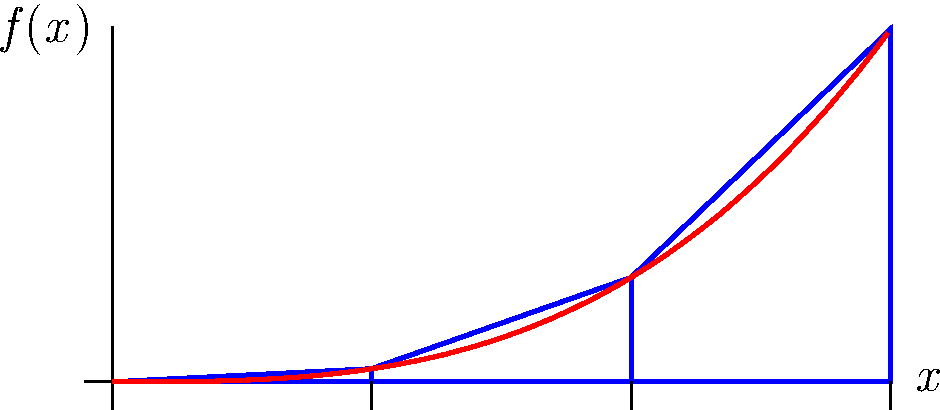
\includegraphics[width=0.7\textwidth]{fig/TrapRiemann.pdf}
\end{center} \pause
\vspace{-2mm}
\begin{align*}
    \mt A_{\eta, a}^{M, 1} = \frac12 \sum_{\kappa = -M}^M \frac{\delta\tau_\kappa}2 \> \big( \e^{-\eta|\tau_\kappa|} \sgn\tau_\kappa \> \e^{-\i \mt H \tau_\kappa} \partial_\lambda \mt H \> \e^{\i \mt H \tau_\kappa} + (\tau_\kappa \leftrightarrow \tau_{\kappa - 1}) \big)
\end{align*} \pause
\vspace{-2mm}
\begin{align*}
    M \geq O(\eta^{-3/2} \epsilon^{-1/2}) \Rightarrow \|(\mt U_{\eta, a} - \mt U_{\eta, a}^{M, 1})\ket{n(\lambdai)}\| \leq \epsilon
\end{align*}
\vspace{-1.4cm}
\end{dia}

\begin{dia}{\lbt}{2. Weighted sum approximation}
This pattern can be continued... \pause
\begin{align*}
    \mt A_{\eta, a}^{M, q} = \frac12 \sum_{\kappa = -M}^M \sum_{\alpha = 0}^q \delta\tau_\kappa w_{\kappa, \alpha} \big( \e^{-\eta|\tau_{\kappa, \alpha}|} \sgn\tau_{\kappa, \alpha} \> \e^{-\i \mt H \tau_{\kappa, \alpha}} \partial_\lambda \mt H \> \e^{\i \mt H \tau_{\kappa, \alpha}}) \big)
\end{align*} \pause
with $\sum_{\alpha = 0}^q w_{\kappa, \alpha} = 1$ \\[6mm] \pause
Weights $w_{\kappa, \alpha}$ only depend on our choice of $\tau_{\kappa, \alpha}$! \\[6mm] \pause
In the end, we get
\begin{align*}
    M \geq O\big( \eta^{-1 - \frac1{q + 1}} \epsilon^{-\frac1{q + 1}} (q + 1)^{-1} \big) \Rightarrow \|(\mt U_{\eta, a} - \mt U_{\eta, a}^{M, q})\ket{n(\lambdai)}\| \leq \epsilon
\end{align*}
\vspace{-0.8cm}
\end{dia}

\begin{dia}{\lbt}{3. Lie-Suzuki-Trotter expansion}
Trotter expansions serve to approximate
\begin{align*}
    \mathcal T \exp[-\i \int_\lambdai^\lambdaf \d\lambda \sum_{\kappa, \alpha} \mt C_{\kappa, \alpha}(\lambda)] 
    \approx \prod_j \exp[-\i \mt C_{\kappa_j, \alpha_j}(\lambda_j) \delta\lambda_j]
\end{align*} \pause
First-order Lie-Suzuki-Trotter (LST) formula:
\begin{align*}
    \tilde{\mt U}_1 = \bigg( \prod_{\kappa=-M}^M \prod_{\alpha = 0}^q \exp \Big[ \!-\!\i \mt C_{\kappa, \alpha} \Big( \lambdai + \frac{\delta\lambda}2 \Big) \frac{\delta\lambda}2 \Big] \bigg) \\\times \bigg( \prod_{\kappa=M}^{-M} \prod_{\alpha = q}^0 \exp \Big[ \!-\!\i \mt C_{\kappa, \alpha} \Big( \lambdai + \frac{\delta\lambda}2 \Big) \frac{\delta\lambda}2 \Big] \bigg)
\end{align*}
where $\delta\lambda = \lambdaf - \lambdai$
\end{dia}

\begin{dia}{\lbt}{3. Lie-Suzuki-Trotter expansion}
We build $k$-th-order LST formulas recursively:
\begin{align*}
\tilde{\mt U}_{k + 1}(\lambdai + \delta\lambda, \lambdai) &= \tilde{\mt U}_k(\lambdai + \delta\lambda, \lambdai + [1 - s_k] \delta\lambda) \\
&\quad \times \tilde{\mt U}_k(\lambdai + [1 - s_k] \delta\lambda, \lambdai + [1 - 2 s_k] \delta\lambda) \nonumber\\
&\quad \times \tilde{\mt U}_k(\lambdai + [1 - 2 s_k] \delta\lambda, \lambdai + 2 s_k \delta\lambda) \\
&\quad \times \tilde{\mt U}_k(\lambdai + 2 s_k \delta\lambda, \lambdai + s_k \delta\lambda) \\
&\quad \times \tilde{\mt U}_k(\lambdai + s_k \delta\lambda, \lambdai)
\end{align*} \pause
If $\mt C(\lambda)$ is sufficiently smooth, then
\begin{align*}
    \| \mathcal T \exp[-\i \int_\lambdai^\lambdaf \d\lambda \sum_{\kappa, \alpha} \mt C_{\kappa, \alpha}(\lambda)] - \tilde{\mt U}_k(\lambdaf, \lambdai) \| \leq O(\delta\lambda^{2k+1})
\end{align*}
\vspace{-1cm}
\end{dia}

\begin{dia}{\lbt}{3. Lie-Suzuki-Trotter expansion}
Error $O(\delta\lambda^{2k + 1})$ is only small when $\delta\lambda = \lambdaf - \lambdai$ is small... \\[4mm] \pause
If not, we divide it into $r$ subintervals so that $O\big( (\delta\lambda / r)^{2k + 1} \big)$ becomes small, and build a product of $r$ LST formulas \\[4mm] \pause
In the end, one can construct a LST formula $\tilde{\mt U}_k$ with
\begin{align*}
    O\bigg( \frac{5^k M \> q}{\eta^{1 + \frac1{2k}}\epsilon^{\frac1{2k}}} \bigg)
\end{align*}
operator exponentials to guarantee 
\begin{align*}
    \| \mathcal T \exp[-\i \int_\lambdai^\lambdaf \d\lambda \sum_{\kappa, \alpha} \mt C_{\kappa, \alpha}(\lambda)] - \tilde{\mt U}_k(\lambdaf, \lambdai) \| \leq \epsilon
\end{align*}
\vspace{-1cm}
\end{dia}

\begin{dia}{\lbt}{Quantum gate complexity}
Lastly, we count the number of quantum gates \\[4mm] \pause
Qubitisation: operator exponential $\exp[-\i \mt H t]$ can be simulated to precision $\delta$ using
\begin{align*}
    O(\|\mt H\|t + \log 1 / \delta)
\end{align*}
elementary quantum gates \\[4mm] \pause
The final gate complexity of our CD algorithm is
\begin{align*}
    %\tilde O\bigg( \frac{5^k (\lambdaf - \lambdai)^{1 + \frac1{2k}}}{\Delta^{3 + \frac3{4k} + \frac3{2(q + 1)}} \epsilon^{1 + \frac3{4k} + \frac3{2(q + 1)}}} \bigg) =
    \tilde O\Big( \Delta^{-3 - \frac3{2(q + 1)}} \epsilon^{-1 - \frac3{2(q + 1)}} \Big) \> \e^{\tilde O\big( \! \sqrt{\log{\frac1{\Delta\epsilon}}} \big)}
\end{align*}
to guarantee $|\bra{n(\lambdaf)} \tilde{\mt U} \ket{n(\lambdai)}|^2 \geq 1 - \epsilon^2$
\vspace{-1cm}
\end{dia}

\begin{dia}{\lbt}{}
\vspace{2.5cm}
\begin{center}
\begin{LARGE}
\textcolor{mygreen}{So what does all of this mean?}
\end{LARGE}
\end{center}
\vspace*{1.5cm}
\end{dia}

\begin{dia}{\lbt}{Conclusion}
Gate-based ASP:
\begin{align*}
    \tilde O(\Delta^{-3} \epsilon^{-1})
\end{align*}
Gate-based CD:
\begin{align*}
    \tilde O\Big( \Delta^{-3 - \frac3{2(q + 1)}} \epsilon^{-1 - \frac3{2(q + 1)}} \Big) \> \e^{\tilde O\big( \! \sqrt{\log{\frac1{\Delta\epsilon}}} \big)}
\end{align*}
where $q$ can be made big cheaply \\[4mm] \pause
Scaling is almost the same for ASP and CD \\[4mm] \pause
``Shortcut to adiabaticity'' turns out not to be much of a shortcut after all...
\end{dia}

\begin{dia}{\lbt}{Conclusion}
Does this mean that CD is useless? \pause No \pause
\begin{itemize}
    \item There might be a better gate-based CD algorithm and/or better bounds \pause
    \item Results only suggest that there may not be much to gain in the worst case \pause
    \item Since CD is basically a coordinate change from time to $\lambda$ space, some kind of ``no free lunch'' phenomenon seems likely \pause
    \item Infidelity estimate $\|(\mt U - \tilde{\mt U})\ket{n(\lambdai}\| \leq \int_\lambdai^\lambdaf \|(\mt A(\lambda) - \tilde{\mt A}(\lambda))\ket{n(\lambda)}\|$ may be easier and more accurate than generic ASP bounds \pause
    \item using simplified AGPs tailored to eigenstate of interest seems promising
\end{itemize}

\vspace{-1cm}
\end{dia}

\begin{dia}{\lbt}{}
\vspace{2.5cm}
\begin{center}
\begin{LARGE}
\textcolor{mygreen}{Questions?}
\end{LARGE}
\end{center}
\vspace*{1.5cm}
\end{dia}

\end{document}